\section{Конструкторский раздел}

\subsection{Проектирование базы данных}

В соответствии с составленной ER-диаграммой системы, проектируемая база данных должна состоять из следующих таблиц:

\begin{itemize}[leftmargin=0.7cm + \labelwidth - \labelsep]
	\item[---] таблица товаров;
	\item[---] таблица поставщиков;
	\item[---] таблица покупателей;
	\item[---] таблица заказов;
	\item[---] таблица пользователей системы.
\end{itemize}

Диаграмма базы данных интернет-магазина представлена на рисунке \ref{konstr:bd}.

\begin{figure}[H]
	\centering{
		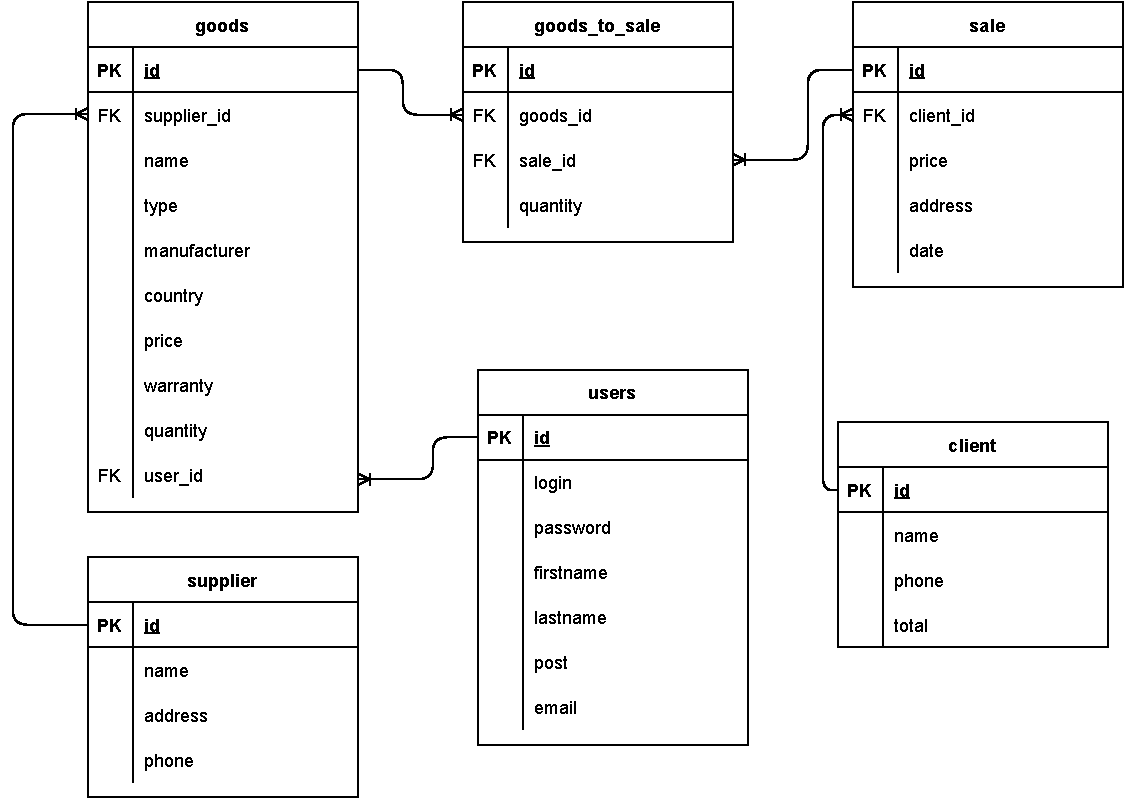
\includegraphics[width=1\textwidth]{img/bd.pdf}
		\caption{Диаграмма базы данных магазина}
		\label{konstr:bd}}
\end{figure}

\subsection{Обновление количества товаров в наличии}

При успешном оформлении заказа покупателем количество товаров в наличии необходимо обновлять. Это действие может выполняться автоматически, если создать соответствующий триггер.

Между таблицей товаров и таблицей заказов существует связь типа «многие-ко-многим», которая реализована с помощью связующей таблицы, в каждой строке которой содержится идентификатор заказа, идентификатор товара и его количество в заказе. Таким образом, чтобы обновить количество у всех товаров, представленных в заказе, можно отслеживать факт добавления новых строк в связующую таблицу.

На рисунке \ref{konstr:updateqnt} представлена схема алгоритма обновления количества товаров в наличии.

\begin{figure}[H]
	\centering{
		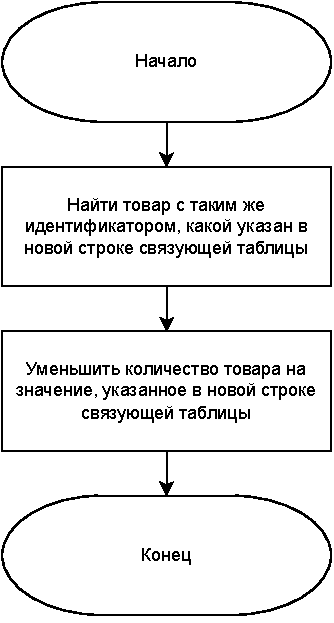
\includegraphics[width=0.4\textwidth]{img/updateqnt.pdf}
		\caption{Алгоритм обновления количества товаров}
		\label{konstr:updateqnt}}
\end{figure}

\subsection{Удаление пользователя системы}

Администратор имеет право удалять пользователей, то есть лишать их возможности авторизации в информационной системе магазина. Это может быть необходимо, например, при увольнении сотрудника. С каждым менеджером магазина связаны товары, которые он добавил в каталог, поэтому имеет смысл сохранять информацию о сотрудниках в базе даже в случае увольнения. В этом случае можно будет отследить все связи и ссылочная целостность базы данных не будет нарушена. Для этого при попытке удаления записи из таблицы пользователей действие можно автоматически заменить на лишение сотрудника должности, а значит, и возможности авторизации в системе.

На рисунке \ref{konstr:deluser} представлена схема алгоритма удаления пользователя системы.

\begin{figure}[H]
	\centering{
		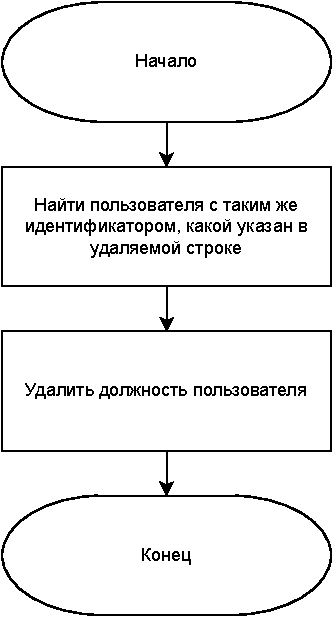
\includegraphics[width=0.4\textwidth]{img/deluser.pdf}
		\caption{Алгоритм удаления пользователя}
		\label{konstr:deluser}}
\end{figure}

\subsection{Ролевая модель}

Создание ролевой модели на уровне базы данных позволяет обеспечить безопасность доступа к её объектам. На уровне базы данных выделены следующие роли:

\begin{itemize}[leftmargin=0.7cm + \labelwidth - \labelsep]
	\item[---] customer -- покупатель;
	\item[---] manager -- менеджер;
	\item[---] admindb -- администратор.
\end{itemize}

\textbf{Покупатель}

Пользователь с ролью customer имеет права на:

\begin{itemize}[leftmargin=0.7cm + \labelwidth - \labelsep]
	\item[---] выборку, изменение в таблице goods;
	\item[---] вставку в таблице goods-to-sale;
	\item[---] выборку, вставку в таблице sale;
	\item[---] выборку, изменение, вставку в таблице client.
\end{itemize}

\textbf{Менеджер}

Пользователь с ролью manager имеет права на:

\begin{itemize}[leftmargin=0.7cm + \labelwidth - \labelsep]
	\item[---] выборку, изменение, вставку в таблице goods;
	\item[---] выборку в таблице goods-to-sale;
	\item[---] выборку в таблице sale;
	\item[---] выборку, вставку в таблице supplier;
	\item[---] выборку в таблице client.
\end{itemize}

\textbf{Администратор}

Пользователь с ролью admindb имеет права на:

\begin{itemize}[leftmargin=0.7cm + \labelwidth - \labelsep]
	\item[---] выборку, изменение, вставку, удаление в таблице users.
\end{itemize}

\subsection*{Вывод}

В данном разделе была представлена диаграмма спроектированной базы данных, описана ролевая модель, а также приведены алгоритмы обновления количества товаров в наличии и удаления пользователя системы.

\pagebreak